\chapter{Architettura e implementazione}
\label{sec:implementazione}

% TODO: AGGIUNGI IMMAGINI, RIFERIMENTI 

% Definire e desccrivere nei dettagli l'architettura a blocchi, descrivendo ciascun blocco e i collegamenti.
% Non è ancora necessario dare dettagli implementativi, che andranno nel capitolo dedicato.
% Descrizione tecnologie utilizzate per implementare ciascun blocco.
% Qui vanno i dettagli implementativi per ciascun blocco dell'architettura definita nel capitolo precedente.
% Potrebbe convenire replicare l'immagine dell'architettura, definendo all'interno dell'immagine dettagli implementativi come ad esempio i nomi dei moduli utilizzati e le tecnologie utilizzate per implementarli.

\section{Sistema di rilevazione anomalie}
Il sistema di rilevazione anomalie, in cui il modulo di correzione è implementato, è costituito dai moduli in figura \ref{fig:sys modules}.
\begin{figure}
    \caption{Architettura del sistema di rilevazione anomalie}
    \label{fig:sys modules}
    \centering
    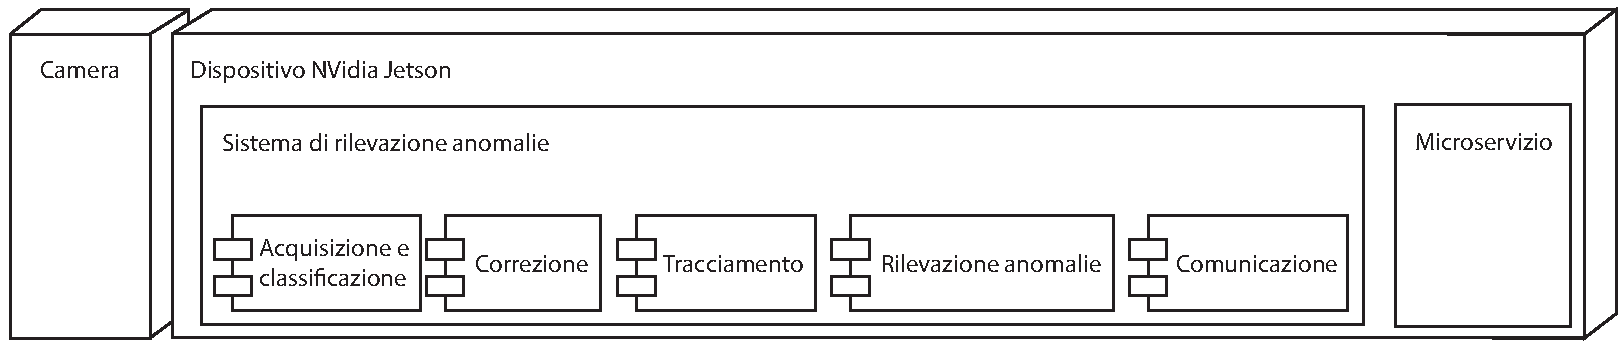
\includegraphics[width=\textwidth]{images/arch.pdf}
\end{figure}
Il sistema è implementato sul dispositivo \emph{Nvidia Jetson Xaxier}\cite{arch:jetson} ed è sviluppato su \emph{Ubuntu 18.04}\cite{arch:ubuntu}.
Il linguaggio di sviluppo è \emph{Python 3.6}\cite{arch:python}.
Per la gestione delle operazione di algebra lineare sono stati utilizzati i package \emph{Numpy}\cite{arch:numpy} e \emph{SciPy}\cite{arch:scipy}.
La pipeline di acquisizione è gestita dalla libreria \emph{GStreamer}\cite{arch:gstreamer}.
La classificazione è effettuata dal modulo di inferenza fornito dall'\emph{SDK Nvidia Deepstream}\cite{arch:deepstream}.
Questo modulo di inferenza è configurato per il modello di \emph{Object Detection YoloV4}\cite{arch:yolo}.

Il modulo di correzione si occupa della rimozione di duplicati ed occlusioni e della correzione della distorsione prospettica descritta in questa tesi.

Il modulo di tracking effettua il tracciamento delle entità, utilizzando una funzione di smoothing per ridurre le imprecisioni della classificazione.
Il tracking è effettuato sia utilizzando l'ultima posizione conosciuta, sia la posizione predetta in base a velocità e accelerazione.

Il modulo di rilevazione di anomalie si occupa di posizionare le entità all'interno della mappa stradale (preconfigurata da un operatore), di assegnarvi una forma approssimata e di comunicare con i sottomoduli di rilevazione delle singole anomalie.
I dati relativi alla mappa sono gestiti attraverso coordinate baricentriche e sono utilizzati per \emph{Cambio di corsia}, \emph{Sosta vietata}, \emph{Persona in strada}, \emph{Invasione di area}.
Gli \emph{Urti} sono verificati simulando la posizione futura delle entità e cercando intersezioni con l'algoritmo \emph{GJK}\cite{arch:gjk}.

Il modulo di comunicazione ottiene i dati relativi alle anomalie e lo stream video e si occupa di salvare segmenti di video in cui sono presenti una o più anomalie.
I dati relativi alle anomalie e il percorso del video sono inviati tramite richiesta HTTP al \emph{Microservizio}, implementato nello stesso dispositivo, che gestisce la comunicazione col backend principale.
Il modulo di comunicazione utilizza \emph{OpenCV}\cite{arch:opencv} per il salvataggio del video e \emph{Requests}\cite{arch:requests} per la comunicazione HTTP.
Il \emph{Microservizio} è implementato con \emph{NodeJS}\cite{arch:nodejs}, \emph{Express}\cite{arch:express}, \emph{Sequelize}\cite{arch:sequelize} e utilizza un database \emph{MySQL}\cite{arch:mysql}.

\section{Strumento interattivo}
Lo strumento interattivo è scritto in \emph{TypeScript}\cite{arch:typescript} e utilizza il framework \emph{SvelteKit}\cite{arch:sveltekit}.
Per le operazioni di algebra lineare è utilizzato \emph{MathJS}\cite{arch:mathjs}.
Per implementare il rendering dell'immagine manipolata è stato utilizzato \emph{GpuJS}\cite{arch:gpujs}, in quanto ha consentito di evitare i costi di tempo richiesti per imparare \emph{WebGL}\cite{arch:webgl}.
Questa libreria non è però abbastanza matura e presenta alcuni comportamenti non ideali, ed è quindi raccomandabile spendere il tempo necessario per imparare \emph{WebGL} in futuro.
Tutto il resto delle funzionalità è implementato attraverso l'uso di \emph{WebAPI}\cite{arch:webapi} e \emph{Svelte}\cite{arch:svelte}.
Il deploy è effettuato come \emph{SPA}\cite{arch:spa} su \emph{GitHub Pages}\cite{arch:ghpages}.
